\section{\texorpdfstring{Phương pháp nghiên cứu}{methodology}}
% Trình bày chi tiết về ý tưởng, các mô hình toán, các chứng minh nếu có. Đồng thời trình bày các bước thực hiện và khảo sát, kiểm nghiệm kết quả nghiên cứu. Mô tả kết quả nghiên cứu khi thử nghiệm với nhiều tập dữ liệu và những độ khó khác nhau.

\subsection{Ý tưởng thực hiện luận văn}

Nhắc lại yêu cầu bài toán: Tạo sinh video khuôn mặt người đang nói dựa trên một hình ảnh tĩnh chứa mặt người mẫu và một đoạn âm thanh chứa tiếng nói. Qua yêu cầu bài toán ta thấy, đầu vào của hệ thống có tính chất khác với đầu ra, sử dụng hình ảnh tĩnh và âm thanh để tạo ra hình ảnh chuyển động. Một số yêu cầu quan trọng khác quyết định chất lượng của chuỗi hình ảnh được tạo sinh ra cũng cần được chú ý. Đó là:
\begin{itemize}
    \item Hình ảnh phải chân thật, rõ ràng, thể hiện được đúng hình dáng gương mặt người đang nói, không bị méo mó, dị dạng.
    \item Chuỗi hình ảnh được tạo sinh cần phải giữ được đặc trưng gương mặt trong ảnh mẫu. Có nghĩa là, người xem vẫn có thể nhận ra được mặt người đang nói trong video được tạo sinh chính là người trong hình ảnh ban đầu
    \item Khẩu hình miệng khi chuyển động phải khớp với âm thanh được nói ra. Sự chuyển động của môi và miệng trong video được tạo sinh phải thể hiện được cách phát âm từ được nói gần như trong thực tế
\end{itemize}

Dựa theo yêu cầu bài toán, ta cần tìm kiếm một phương pháp để kết hợp đặc trưng âm thanh và hình ảnh lại với nhau, sau đó chuyển đổi đặc trưng này thành video. Để mang lại sự trung thực, sắc nét cho hình ảnh được tạo sinh cũng như lưu giữ được các đặc trưng khuôn mặt người trong hình ảnh ban đầu, chiến thuật của ta là sẽ dựa hoàn toàn trên hình ảnh ban đầu để tạo sinh các khung hình khác trong video. Như vậy, với mỗi khung hình ở mỗi thời điểm $t$ trên video, ta cần phải tìm kiếm sự thay đổi của khung ảnh tại thời điểm đó so với hình ảnh tĩnh được cho ban đầu. Sau đó, ta thực hiện biến đổi hình ảnh được cho ban đầu thành hình ảnh ở khung hình tại thời điểm $t$. Như vậy, câu hỏi đặt ra là ta cần phải thay đổi tại vùng nào trên ảnh mẫu và tại những vùng đó ta sẽ thay đổi như thế nào, thay đổi nhiều hay ít.

Sự thay đổi của hình ảnh được quyết định phần nhiều bởi chuỗi âm thanh được đưa vào hệ thống. Âm thanh giọng nói quyết định khẩu hình miệng và các biểu cảm trên gương mặt. Đôi khi, giọng nói còn có thể quyết định cách chuyển động của đầu. Tuy nhiên, tuy giọng nói góp phần lớn khi định hình sự thay đổi trên gương mặt trong lúc nói, ảnh mẫu ban đầu cũng quyết định phần nào các thay đổi đó. Hình ảnh ban đầu cung cấp thông tin về nhận dạng khuôn mặt, về những đặc điểm của các bộ phận trên gương mặt người nói, về vị trí của mắt, mũi, miệng để định hình cách âm thanh thay đổi hình dạng gương mặt trong lúc nói.

\begin{figure}[H]
    \centering
    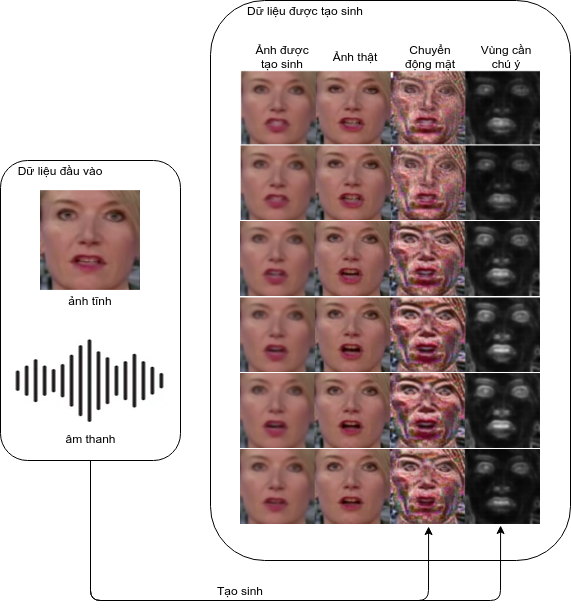
\includegraphics[width=12cm]{./content/materials/idea.png}
    \caption{Ý tưởng về tạo sinh chuỗi hình ảnh chuyển động cho mặt người đang nói}
\end{figure}

Ý tưởng giải quyết bài toán được thể hiện ở hình trên. Chúng ta sẽ tạo ra một hệ thống có khả năng trích xuất đặc trưng của hình ảnh tĩnh ban đầu và âm thanh giọng nói để tạo ra hình ảnh chuyển động của mặt. Tuy nhiên, hình ảnh chuyển động mặt này không hoàn toàn được sử dụng, mà song song với nó, ta tạo ra một mặt nạ tương ứng. Mặt nạ này chỉ chú ý tới một số khu vực trên hình ảnh chuyển động mặt được tạo sinh. Những vùng màu đen là những vùng không được chú ý đến trên ảnh chuyển động vừa được sinh ra, ngược lại, các vùng có màu trắng càng sáng thì càng được chú ý. Như vậy, mặt nạ chú ý sẽ cho ta biết ta nên thay đổi những vùng nào trên gương mặt tại thời điểm $t$ tương ứng với tiếng nói ở thời điểm đó. Đồng thời, hình ảnh chuyển động mặt được tạo sinh song song cho ta biết ta phải thay đổi như thế nào ở những điểm được chú ý. Ở những điểm không được chú ý còn lại, ta sẽ thay thế bằng các điểm ảnh trong ảnh gốc ban đầu. Nhờ vậy, ta có thể bảo toàn được nhận dạng của người nói trong quá trình tạo sinh bằng việc chỉ tìm ra những điểm thay đổi trên gương mặt thay vì cố gắng tìm cách tạo sinh toàn bộ gương mặt của người nói.

\subsection{Mô hình hóa bài toán}

\begin{figure}[H]
    \centering
    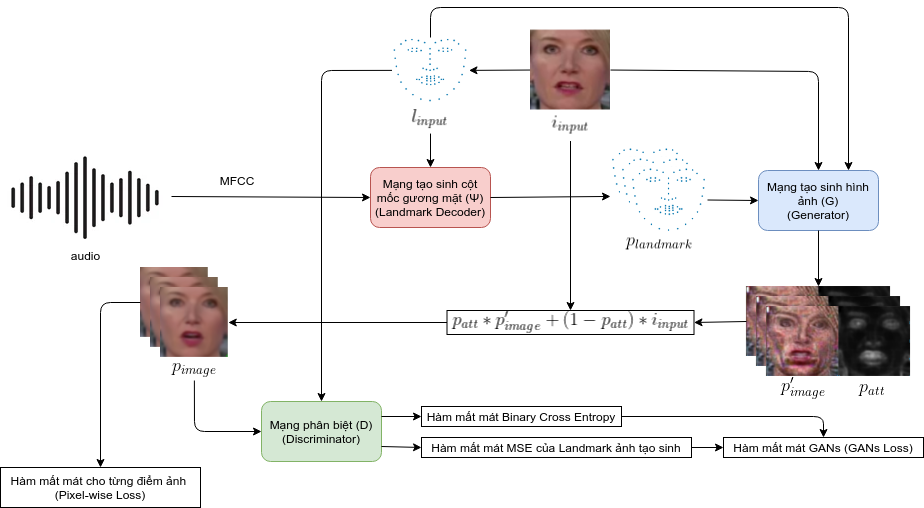
\includegraphics[width=15cm]{./content/materials/common_architecture.png}
    \caption{Cấu trúc chung của hệ thống}
\end{figure}

\subsection{Các tập dữ liệu được sử dụng}
\subsubsection{Tập dữ liệu GRID \cite{grid}}

\begin{figure}[H]
    \centering
    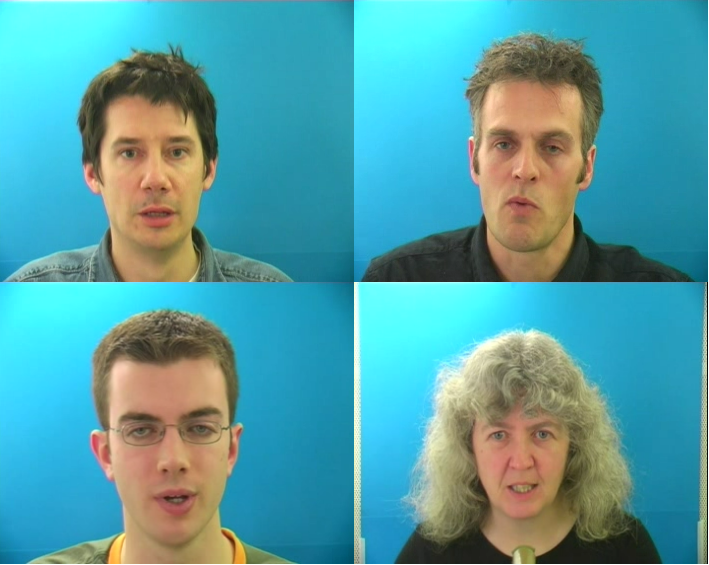
\includegraphics[width=12cm]{./content/materials/grid.png}
    \caption{Ảnh trích xuất từ các video trong tập dữ liệu GRID}
\end{figure}

\subsubsection{Tập dữ liệu LRW \cite{lrw}}

\begin{figure}[H]
    \centering
    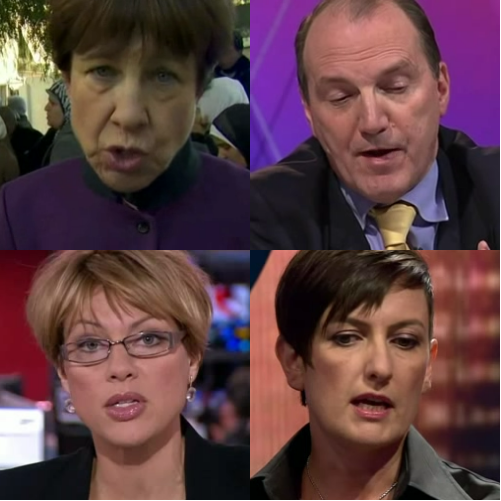
\includegraphics[width=12cm]{./content/materials/lrw.png}
    \caption{Ảnh trích xuất từ các video trong tập dữ liệu LRW}
\end{figure}

\subsection{Tiền xử lý dữ liệu}

\subsection{Cấu trúc tổng quát của hệ thống}

\subsection{Cấu trúc của bộ giải mã landmark của khuôn mặt (Landmark Decoder)}

\begin{figure}[H]
    \centering
    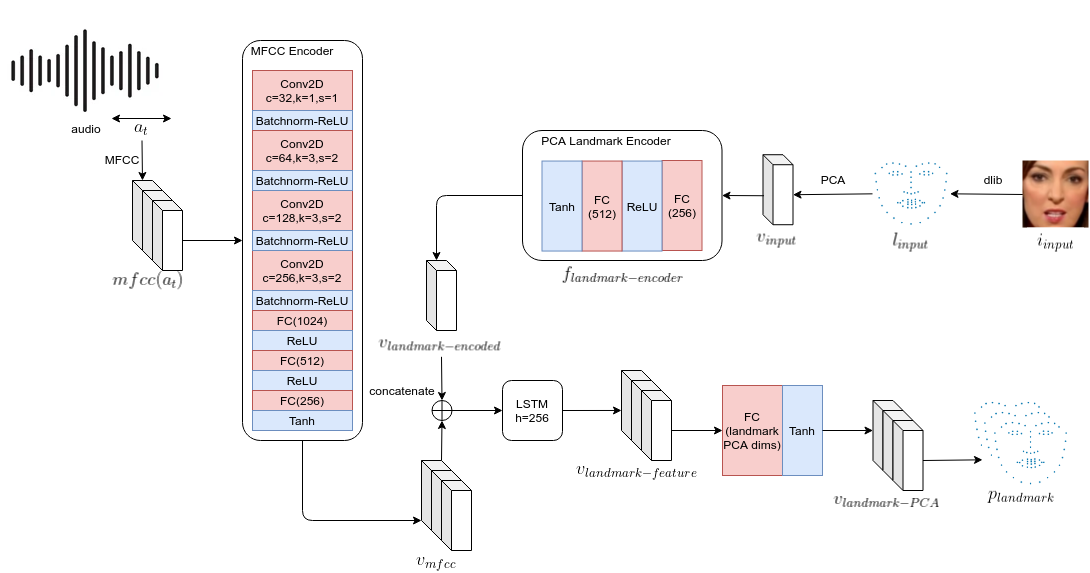
\includegraphics[width=15cm]{./content/materials/landmark_decoder.png}
    \caption{Cấu trúc của bộ giải mã landmark của khuôn mặt (Landmark Decoder)}
\end{figure}

\subsection{Cấu trúc của bộ tạo sinh hình ảnh (Generator)}

\begin{figure}[H]
    \centering
    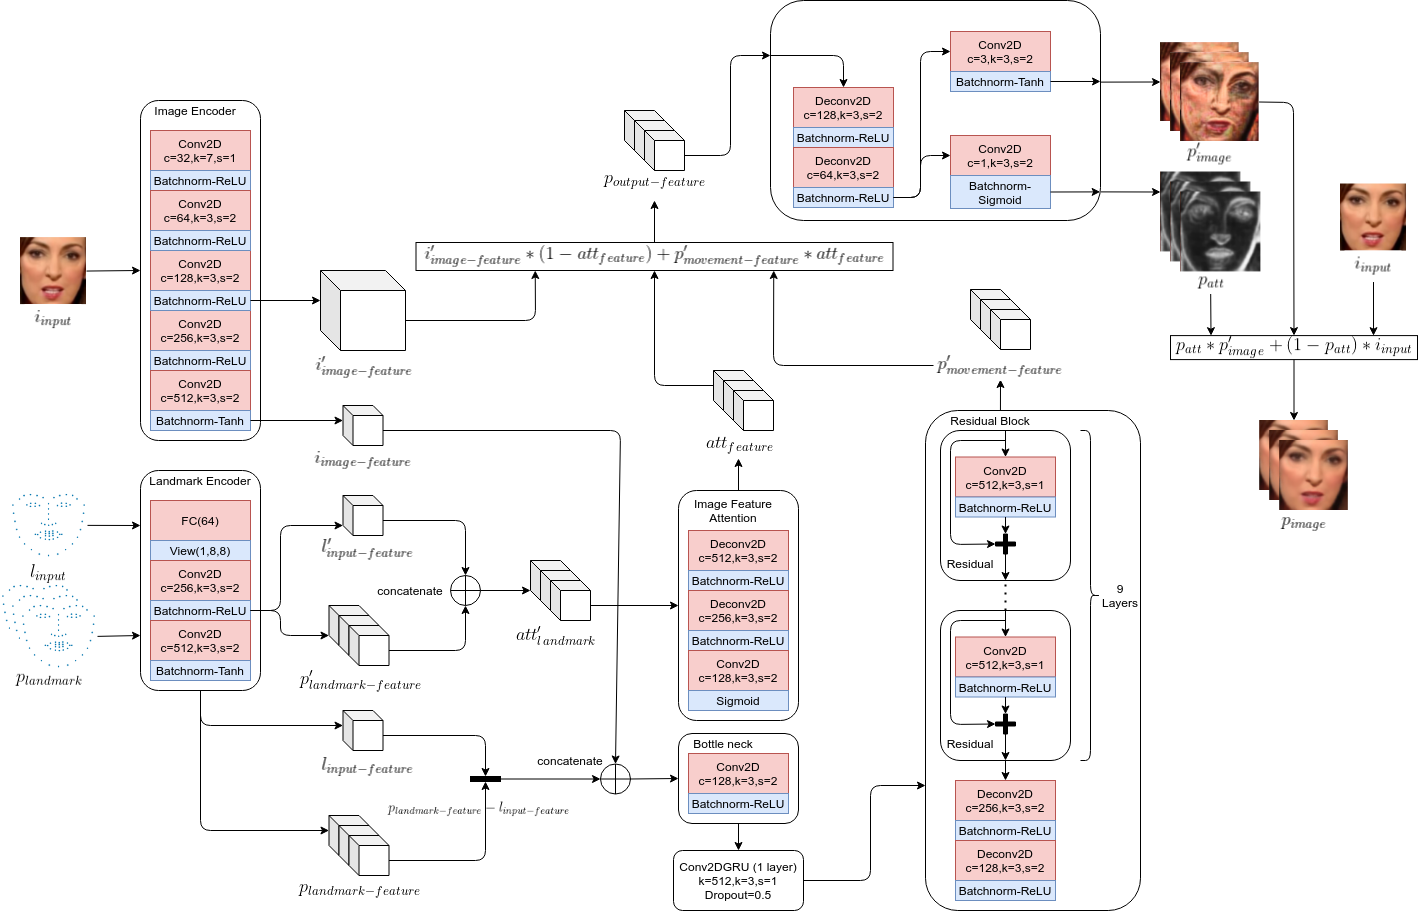
\includegraphics[width=15cm]{./content/materials/generator.png}
    \caption{Cấu trúc của bộ giải mã landmark của khuôn mặt (Generator)}
\end{figure}

\subsection{Cấu trúc của bộ phân biệt hình ảnh (Discriminator)}

\begin{figure}[H]
    \centering
    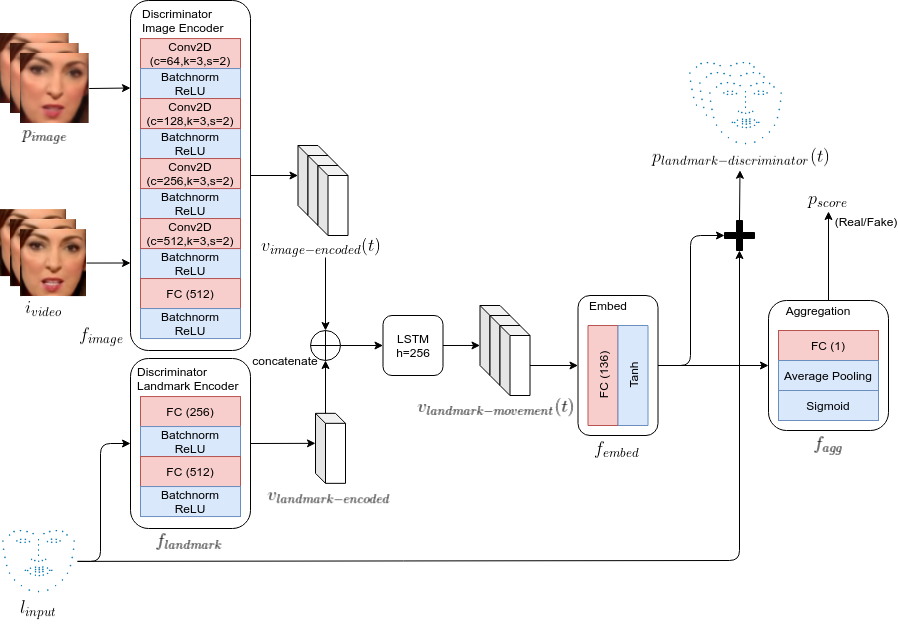
\includegraphics[width=15cm]{./content/materials/discriminator.png}
    \caption{Cấu trúc của bộ phân biệt hình ảnh (Discriminator)}
\end{figure}

\subsection{Hàm mất mát được sử dụng cho hệ Generator - Discriminator}
